\documentclass[12pt]{article}
\usepackage[margin=2.5cm]{geometry}
\usepackage{enumerate}
\usepackage{amsfonts}
\usepackage{amsmath}
\usepackage{fancyhdr}
\usepackage{amsmath}
\usepackage{amssymb}
\usepackage{amsthm}
\usepackage{mdframed}
\usepackage{graphicx}
\usepackage{subcaption}

\begin{document}
\title{Worksheet 19 Solution}
\author{Hyungmo Gu}
\maketitle

\section*{Question 1}
\begin{enumerate}[a.]
    \item
    By the figure below, we can conclude there are 7 vertices.

    \begin{center}
    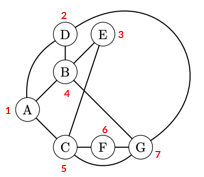
\includegraphics[width=6cm]{images/worksheet_19_q1a_solution.png}
    \end{center}

    \item
    By the figure below, we can conclude there are 11 edges.

    \begin{center}
    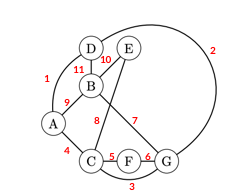
\includegraphics[width=6cm]{images/worksheet_19_q1b_solution.png}
    \end{center}

    \newpage
    \item
    By the figure below, we can conclude there are 4 vertices adjacent to G.

    \begin{center}
    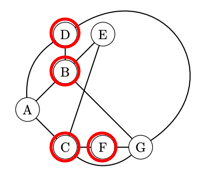
\includegraphics[width=6cm]{images/worksheet_19_q1c_solution.png}
    \end{center}

    \item
    By the figure below, we can conclude the distance between A ang G is 2.

    \begin{center}
    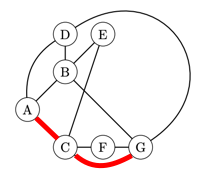
\includegraphics[width=6cm]{images/worksheet_19_q1d_solution.png}
    \end{center}

    \bigskip

    There are 2 shortest paths between A and G. One is the path from A to C to G as
    shown above, and the other is the path from A to B to G

    \begin{center}
    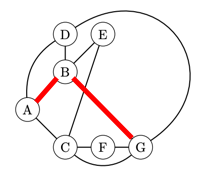
\includegraphics[width=6cm]{images/worksheet_19_q1d2_solution.png}
    \end{center}

    \begin{mdframed}
        \underline{\textbf{Correct Solution:}}

        By the figure below, we can conclude the distance between A ang G is 2.

        \begin{center}
        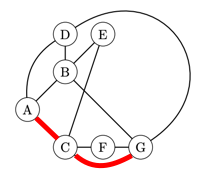
\includegraphics[width=6cm]{images/worksheet_19_q1d_solution.png}
        \end{center}

        \bigskip

        There are \color{red}3\color{black}\:shortest paths between A and G. One
        is the path from A to C to G as shown above, and the other is the path
        from A to B to G

        \begin{center}
        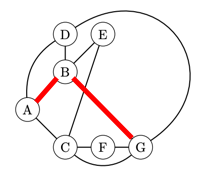
\includegraphics[width=6cm]{images/worksheet_19_q1d2_solution.png}
        \end{center}

        \color{red}
        and the last one is from A to D to G

        \begin{center}
        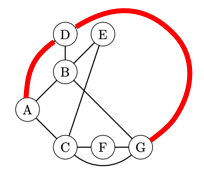
\includegraphics[width=6cm]{images/worksheet_19_q1d3_solution.png}
        \end{center}
        \color{black}
    \end{mdframed}

    \bigskip

    \textbf{Notes:}

    \begin{itemize}
     \item \textbf{Distance} is the number of edges in a shortest path.
    \end{itemize}

    \item Path [C,F,G,D,A,B,E] is one example that goes through all vertices of
    the graph.

    \begin{center}
    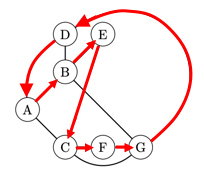
\includegraphics[width=6cm]{images/worksheet_19_q1e_solution.png}
    \end{center}

\end{enumerate}

\section*{Question 2}
\begin{enumerate}[a.]
    \item By the figure below, we can conclude the degree of vertex D is 3.

    \begin{center}
    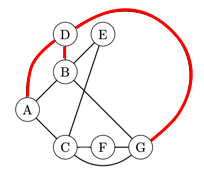
\includegraphics[width=6cm]{images/worksheet_19_q2a_solution.png}
    \end{center}

    \item By the figure below, we can see

    \begin{itemize}
        \item vertex A has degree of 3
        \item vertex B has degree of 4
        \item vertex C has degree of 4
        \item vertex D has degree of 3
        \item vertex E has degree of 2
        \item vertex F has degree of 2
        \item vertex G has degree of 4
    \end{itemize}

    \bigskip

    Using this fact, we can conclude the vertices with the largest degree are
    B,C and G.

    \begin{figure}[h]
        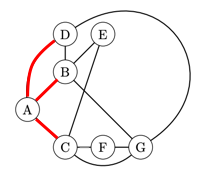
\includegraphics[width=0.24\textwidth]{images/worksheet_19_q2b1_solution.png}\hfill
        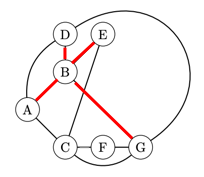
\includegraphics[width=0.24\textwidth]{images/worksheet_19_q2b2_solution.png}\hfill
        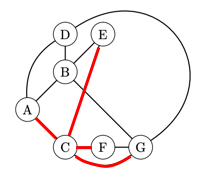
\includegraphics[width=0.24\textwidth]{images/worksheet_19_q2b3_solution.png}\hfill
        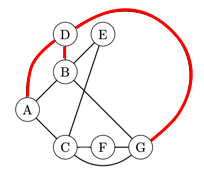
\includegraphics[width=0.24\textwidth]{images/worksheet_19_q2b4_solution.png}\hfill
        \\
        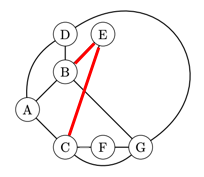
\includegraphics[width=0.24\textwidth]{images/worksheet_19_q2b5_solution.png}\hfill
        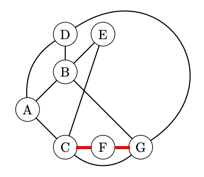
\includegraphics[width=0.24\textwidth]{images/worksheet_19_q2b6_solution.png}\hfill
        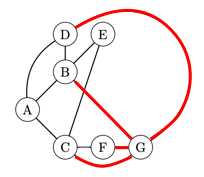
\includegraphics[width=0.24\textwidth]{images/worksheet_19_q2b7_solution.png}\hfill
        
\includegraphics[width=0.24\textwidth]{images/worksheet_19_q2b8_placeholder.png}\hfill
    \end{figure}

    \newpage

    \item

    \textbf{Statement:} $\forall G = (V,E),\:(\forall v \in V,\:d(v) \leq 5)
    \Rightarrow \lvert E \rvert \leq \frac{5}{2} \lvert V \rvert$

    \bigskip

    \begin{proof}

        Let $G = (V,E)$ be a graph. Assume $v \in V$ and $d(v) \leq 5$.

        \bigskip

        We need to show $\lvert E \rvert \leq \frac{5}{2} \lvert V \rvert$.

        \bigskip

        Because we know the number of edges is half of the summation of all
        degrees of v in V, we can write

        \begin{align}
            \lvert E \rvert &= \frac{1}{2} \cdot \sum\limits_{v \in V} d(v)
        \end{align}

        \bigskip

        Then, using the assumption $d(v) \leq 5$, we can conclude

        \begin{align}
            \lvert E \rvert &\leq \frac{1}{2} \cdot \sum\limits_{v \in V} 5\\
            &= \frac{5}{2} \lvert V \rvert
        \end{align}
    \end{proof}

    \bigskip

    \textbf{Notes:}

    \begin{itemize}
     \item I should work on improving this proof in future iterations. I feel
     the beginning has been jumped too quick.

    \end{itemize}

\end{enumerate}

\section*{Question 3}
\begin{enumerate}[a.]
    \item

    The adjacency matrix of this graph is

    \setcounter{equation}{0}
    \begin{align}
    \begin{bmatrix}
    0 & 1 & 0 & 1 & 0\\
    1 & 0 & 1 & 0 & 1\\
    0 & 1 & 0 & 0 & 1\\
    1 & 0 & 0 & 0 & 1\\
    0 & 1 & 1 & 1 & 0
    \end{bmatrix}
    \end{align}
\end{enumerate}

\end{document}